\documentclass{article}

\usepackage{mathptmx}
%packages for language
\usepackage[czech]{babel}
\usepackage[utf8]{inputenc}
%packages for graphic
\usepackage{graphicx}
\usepackage{pgfplots}
\usepackage{pgfplotstable}
\usepackage{multirow}
\usepackage{tikz}
\usepackage{import}
\usepackage[a4paper, total={17cm,25.7cm}, top=2cm, left=2cm, includefoot]{geometry}
\usepackage{todonotes}
\usepackage{standalone}
\usepackage{colortbl}%pro barevne zmeny v tabulce
\usepackage{float}
\usepackage{csvsimple} %pro import a práci s csv soubory
\usepackage{indentfirst}  % odsazení prvního řádku v odstavci
\usepackage{hyperref} %dela odkazy na mista v dokumentu atd
\usepackage{amsmath}%psani matic
\usepackage{mathrsfs}%psani kroucenym matematickym pismem
\usepackage{pdfpages}%vkladani celych pdf dokumentu
%cesta k obrazkum: ./Graphics/....

\begin{document}
	\begin{titlepage}
    \begin{center}
        \LARGE
        Západočeská Univerzita v Plzni\\
        Fakulta Aplikovaných Věd\\
        
        \vspace{1cm}
        
        
\includegraphics[width=0.5\textwidth]{./Graphics/FAV_logo.pdf}
        
        \vspace{4cm}
        
        \textbf{Markovské řetězce}
        
        \vspace{0.5cm}
        Semestrální práce č. 1
        
        \vspace{0.5cm}
        Filip Jašek
        
    \end{center} 
    \vfill
        \noindent
        \large
        Předmět: KKY/STP (Stochastické Systémy a Procesy)\\
        Přednášející: Doc. Ing. Straka Ondřej, Ph.D.\\
        Cvičící: Ing. Kost Oliver\hfill Datum: \today
\end{titlepage}
	
	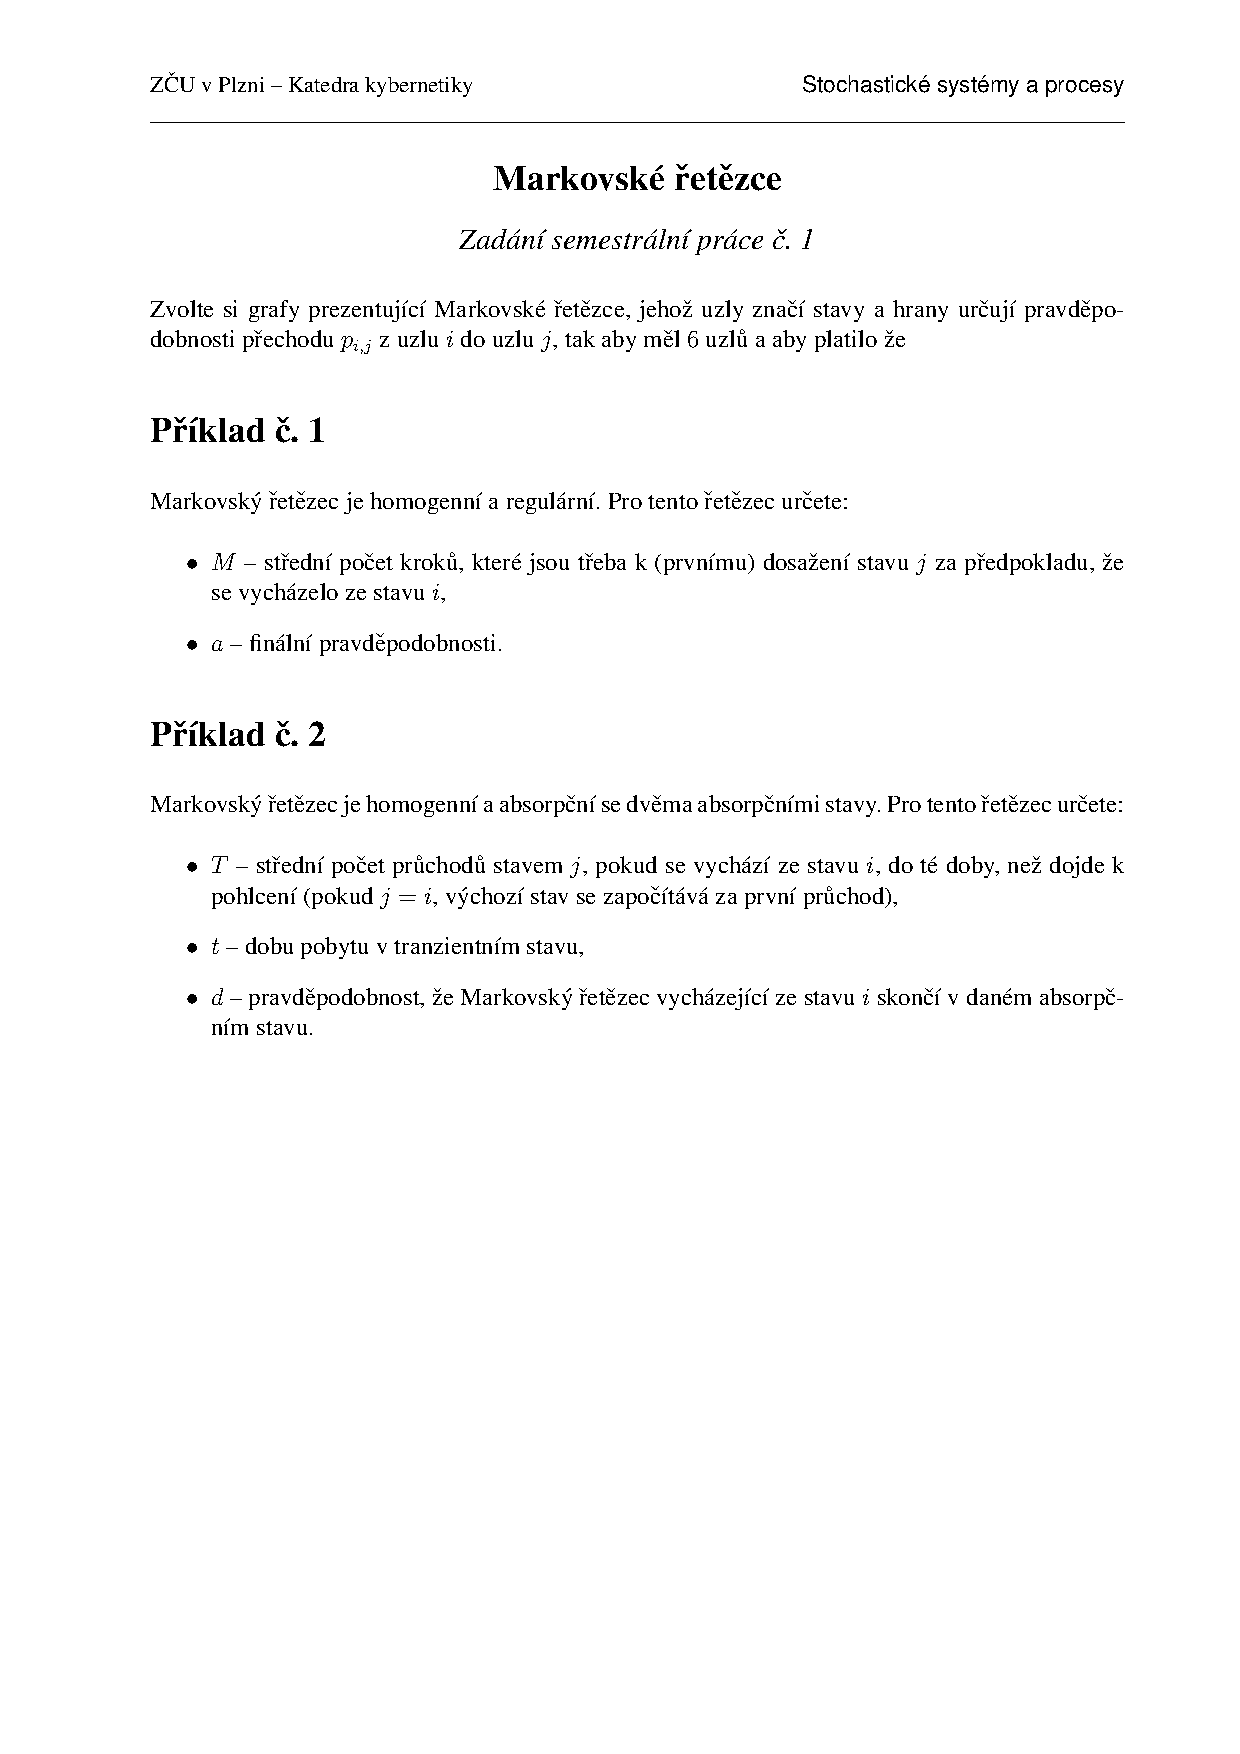
\includepdf[scale=0.85,pages=1, pagecommand=\section{Zadání}\centering]{./Graphics/STP_semestralka01_zadani.pdf}
	
	\section{Příklad č. 1}
		Pro zadaná kritéria byl vytvořen homogenní regulární Markovský řetězec zobrazen na obrázku \ref{pic:markovsky_retezec_obr} s přechodovou maticí
		\[P = \begin{bmatrix}
			\frac{1}{2}&\frac{1}{2}&0&0&0&0\\
			0&\frac{1}{2}&\frac{1}{2}&0&0&0\\
			0&0&\frac{1}{2}&\frac{1}{2}&0&0\\
			0&0&0&\frac{1}{2}&\frac{1}{2}&0\\
			0&0&0&0&\frac{1}{2}&\frac{1}{2}\\
			\frac{1}{2}&0&0&0&0&\frac{1}{2}
		\end{bmatrix}\]
			\begin{figure}[H]
				\centering
				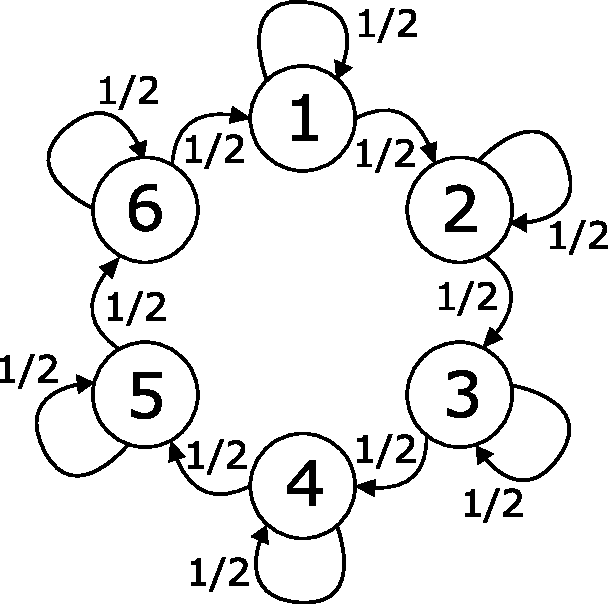
\includegraphics[width=.5\textwidth]{./Graphics/priklad_01.pdf}
				\caption{Graf zvoleného Markovského řetězce.}
				\label{pic:markovsky_retezec_obr}
			\end{figure}
		\subsection{Střední počet kroků ze stavu \(i\) do \(j\)}
			Pro zjištění středního počtu kroků k dosažení stavu \(j\) za předpokladu vycházení ze stavu \(i\) lze použít vztah \[m_{ij}=\sum_{s=1}^{\infty}p_{is}\cdot m_{sj}+1\] nebo jeho maticový zápis \[\mathbf{M}=\mathbf{P}\overline{\mathbf{M}}+\mathbf{E},\]kde matice \(\mathbf{M}\) je matice prvků \(m_{ij}\), \(\overline{\mathbf{M}}\) je matice \(\mathbf{M}\), kde na hlavní diagonále (pozice \(i=j\)) jsou nuly a \(\mathbf{E}\) je matice s jedničkami na všech pozicích.\\
			
			Za pomoci symbolického výpočtu v Matlabu jsme docílili následujícího výsledku.
			\[\mathbf{M}=\mathbf{P}\overline{\mathbf{M}}+\mathbf{E}
			\begin{bmatrix}
				m_{11}&m_{12}&m_{13}&m_{14}&m_{15}&m_{16}\\
				m_{21}&m_{22}&m_{23}&m_{24}&m_{25}&m_{26}\\
				m_{31}&m_{32}&m_{33}&m_{34}&m_{35}&m_{36}\\
				m_{41}&m_{42}&m_{43}&m_{44}&m_{45}&m_{46}\\
				m_{51}&m_{52}&m_{53}&m_{54}&m_{55}&m_{56}\\
				m_{61}&m_{62}&m_{63}&m_{64}&m_{65}&m_{66}
			\end{bmatrix}=\] 
			\[=\begin{bmatrix}
				\frac{1}{2}&\frac{1}{2}&0&0&0&0\\
				0&\frac{1}{2}&\frac{1}{2}&0&0&0\\
				0&0&\frac{1}{2}&\frac{1}{2}&0&0\\
				0&0&0&\frac{1}{2}&\frac{1}{2}&0\\
				0&0&0&0&\frac{1}{2}&\frac{1}{2}\\
				\frac{1}{2}&0&0&0&0&\frac{1}{2}
			\end{bmatrix}\cdot
			\begin{bmatrix}
				0&m_{12}&m_{13}&m_{14}&m_{15}&m_{16}\\
				m_{21}&0&m_{23}&m_{24}&m_{25}&m_{26}\\
				m_{31}&m_{32}&0&m_{34}&m_{35}&m_{36}\\
				m_{41}&m_{42}&m_{43}&0&m_{45}&m_{46}\\
				m_{51}&m_{52}&m_{53}&m_{54}&0&m_{56}\\
				m_{61}&m_{62}&m_{63}&m_{64}&m_{65}&0
			\end{bmatrix} + 
			\begin{bmatrix}
				1&1&1&1&1&1\\
				1&1&1&1&1&1\\
				1&1&1&1&1&1\\
				1&1&1&1&1&1\\
				1&1&1&1&1&1\\
				1&1&1&1&1&1\\
			\end{bmatrix}=\]
			\[=\begin{bmatrix}
				6&2&4&6&8&10\\
				10&6&2&4&6&8\\
				8&10&6&2&4&6\\
				6&8&10&6&2&4\\
				4&6&8&10&6&2\\
				2&4&6&8&10&6
			\end{bmatrix}\]
		\subsection{Finální pravděpodobnost}
			Finální pravděpodobnost se získá limitou mocniny přechodové matice do \(\infty\).
			\[\mathbf{P}_{final} = \lim_{k \to \infty}\mathbf{P}^{k}=
			\begin{bmatrix}
				0.1667&0.1667&0.1667&0.1667&0.1667&0.1667\\
				0.1667&0.1667&0.1667&0.1667&0.1667&0.1667\\
				0.1667&0.1667&0.1667&0.1667&0.1667&0.1667\\
				0.1667&0.1667&0.1667&0.1667&0.1667&0.1667\\
				0.1667&0.1667&0.1667&0.1667&0.1667&0.1667\\
				0.1667&0.1667&0.1667&0.1667&0.1667&0.1667
			\end{bmatrix}\]
		
	\newpage	
	\section{Příklad č. 2}
		Pro následující výpočty byl vytvořen nový homogenní absorpční Markovský řetězec s dvěma absorpčními stavy zakreslený na obrázku \ref{pic:markovsky_retezec_obr_2}, popsaný maticí přechodu
		\[\mathbf{P} = \begin{bmatrix}
			1	&0	&0	&0	&0	&0\\
			1/3	&0	&0	&0	&2/3&0\\
			0	&2/3&0	&1/3&0	&0\\
			0	&0	&0	&1	&0	&0\\
			0	&0	&0	&1/3&0	&2/3\\
			1/3	&0	&2/3&0	&0	&0
		\end{bmatrix}\]
		
			\begin{figure}[H]
				\centering
				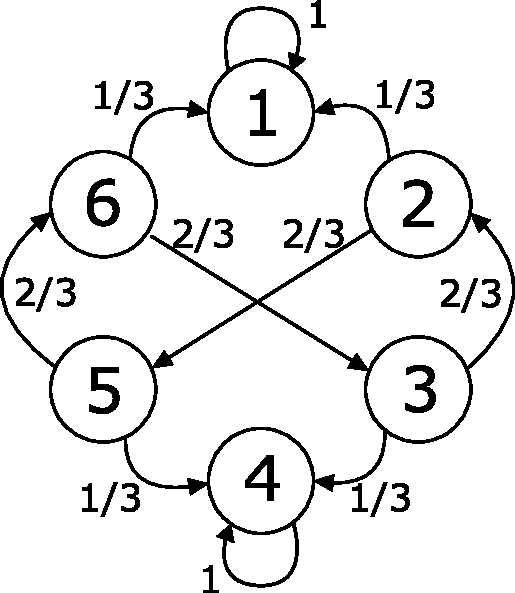
\includegraphics[width=.5\textwidth]{./Graphics/priklad_02.pdf}
				\caption{Graf druhého zvoleného Markovského řetězce s dvěma absorpčními stavy.}
				\label{pic:markovsky_retezec_obr_2}
			\end{figure}
		\subsection{Střední počet průchodů stavem \(j\)}
			Při startu ze stavu \(i\) spočteme střední počet průchodů tranzientním stavem \(j\) před pohlcením vztahem \[\mathbf{T} = (\mathbf{I}-\mathbf{Q})^{-1},\] kde \(\mathbf{Q}\) získáme z matice \(\mathbf{P}\) vynecháním řádků a sloupců odpovídající absorpčním stavům a \(I\) jako jednotkovou matici.
			\[\mathbf{T} = (\mathbf{I}-\mathbf{Q})^{-1}=
			\left(
			\begin{bmatrix}
				1&0&0&0\\
				0&1&0&0\\
				0&0&1&0\\
				0&0&0&1
			\end{bmatrix}-
			\begin{bmatrix}
				0&0&\frac{2}{3}&0\\
				\frac{2}{3}&0&0&0\\
				0&0&0&\frac{2}{3}\\
				0&\frac{2}{3}&0&0
			\end{bmatrix}
			\right)^{-1}=
			\begin{bmatrix}
				1.2462&    0.3692&    0.8308&    0.5538\\
				0.8308&    1.2462&    0.5538&    0.3692\\
				0.3692&    0.5538&    1.2462&    0.8308\\
				0.5538&    0.8308&    0.3692&    1.2462
			\end{bmatrix}\]
		\subsection{Doba pobytu v tranzientním stavu}
			Dobu pobytu v tranzientím stavu zjistíme za pomoci vztahu \[\mathbf{t}=\mathbf{T}\cdot \mathbf{E},\] kde \(\mathbf{T}\) je matice středního počtu průchodů vypočtená v předchozím příkladu a \(\mathbf{E}\) je vektor jedniček.
			\[\mathbf{t} = \mathbf{T}\cdot \mathbf{E}=
			\begin{bmatrix}
				1.2462&    0.3692&    0.8308&    0.5538\\
				0.8308&    1.2462&    0.5538&    0.3692\\
				0.3692&    0.5538&    1.2462&    0.8308\\
				0.5538&    0.8308&    0.3692&    1.2462
			\end{bmatrix}\cdot
			\begin{bmatrix}
				1\\
				1\\
				1\\
				1
			\end{bmatrix}=
			\begin{bmatrix}
				3\\
				3\\
				3\\
				3
			\end{bmatrix}\]
		\subsection{Pravděpodobnost konce v absorpčním stavu}
			Pravděpodobnost konce v jednom z absorpčních stavů je dána vztahem \[\mathbf{d}=\mathbf{T}\cdot \mathbf{R},\] kde \(\mathbf{T}\) je již vypočtená matice středního počtu průchodů a \(\mathbf{R}\) je část matice přechodu \(\mathbf{P}\). \(\mathbf{R}\) tedy bude obsahovat řádky bez absorpčních stavů a sloupce pouze absorpčních stavů.
			\[\mathbf{d}=\mathbf{T}\cdot \mathbf{R}=
			\begin{bmatrix}
				1.2462&    0.3692&    0.8308&    0.5538\\
				0.8308&    1.2462&    0.5538&    0.3692\\
				0.3692&    0.5538&    1.2462&    0.8308\\
				0.5538&    0.8308&    0.3692&    1.2462
			\end{bmatrix}\cdot
			\begin{bmatrix}
				\frac{1}{3}&0\\
				0&\frac{1}{3}\\
				0&\frac{1}{3}\\
				\frac{1}{3}&0
			\end{bmatrix}=
			\begin{bmatrix}
				0.6    &0.4\\
				0.4    &0.6\\
				0.4    &0.6\\
				0.6    &0.4
			\end{bmatrix}\]
	\newpage
	\section{Závěr}
		Vzorce byly čerpány z přednášek a výpočty byly provedeny za pomoci softwaru Matlab. Samotné vypracování práce mi pomohlo lépe pochopit Markovské řetězce a jejich parametry.
\end{document}
